\begin{figure}[ht]
\centering
\resizebox{0.9\linewidth}{!}{%
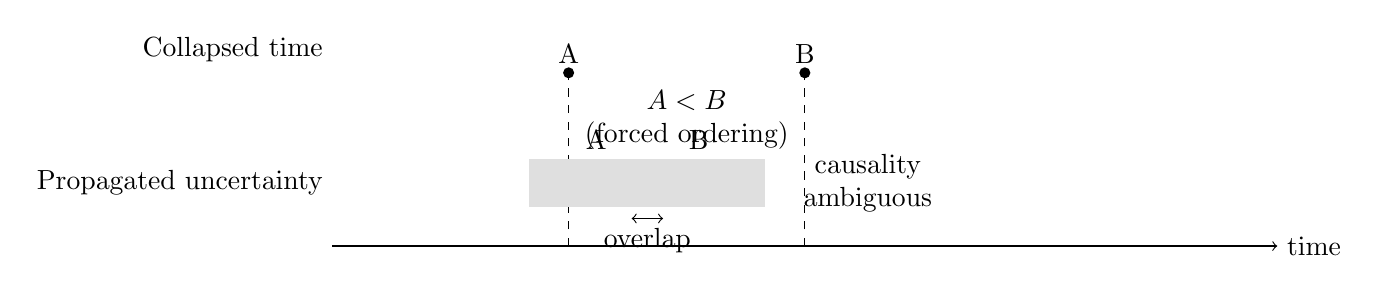
\begin{tikzpicture}[x=1cm,y=1cm]

% Time axis
\draw[->] (0,0) -- (12,0) node[right]{time};

% Labels
\node[anchor=east] at (0,2.5) {Collapsed time};
\node[anchor=east] at (0,0.8) {Propagated uncertainty};

% --- Collapsed representation ---
% Event A
\draw[dashed] (3,0) -- (3,2.2);
\fill (3,2.2) circle (2pt);
\node[above] at (3,2.2) {A};

% Event B
\draw[dashed] (6,0) -- (6,2.2);
\fill (6,2.2) circle (2pt);
\node[above] at (6,2.2) {B};

\node[align=center] at (4.5,1.6) {$A < B$\\(forced ordering)};

% --- Interval representation ---
% Event A interval
\draw[fill=gray!25,draw=none] (2.5,0.5) rectangle (4.2,1.1);
\node[above] at (3.35,1.1) {A};

% Event B interval
\draw[fill=gray!25,draw=none] (3.8,0.5) rectangle (5.5,1.1);
\node[above] at (4.65,1.1) {B};

% Overlap annotation
\draw[<->] (3.8,0.35) -- (4.2,0.35);
\node[below] at (4.0,0.35) {overlap};

\node[align=center] at (6.8,0.8) {causality\\ambiguous};

\end{tikzpicture}
}
\caption{Temporal causality under collapsed versus propagated time. When timestamps are collapsed to points (top), events appear totally ordered even when that ordering is not justified; when uncertainty is propagated (bottom), overlapping event intervals make causal ambiguity explicit and queryable.}
\end{figure}